\documentclass[11pt]{article}
\usepackage[a4paper, top=2.5cm, bottom=2.5cm, left=2.5cm, right=2.5cm]{geometry}
\usepackage{amsmath, amssymb}
\usepackage{xcolor}
\usepackage{graphicx}
\usepackage{tikz}
\usetikzlibrary{arrows.meta, decorations.pathmorphing, quantikz2}
\usepackage{pgfplots}
\pgfplotsset{compat=1.18}
\usepackage{circuitikz}
\usepackage{tikz-cd}
\definecolor{tdc1}{HTML}{6B6B6B}
\definecolor{tdc2}{HTML}{E8F0FB}
\definecolor{tdc3}{HTML}{E6F4EA}
\definecolor{tdc4}{HTML}{A05A5A}
\definecolor{tdc5}{HTML}{1E5BD6}
\definecolor{tdc6}{HTML}{D62728}
\definecolor{tdc7}{HTML}{1E63C4}

\title{Welcome to DiagramTeX}
\date{}

\begin{document}
\maketitle

Draw figures for \LaTeX\ and export them as TikZ, SVG, PNG or PDF. Your work saves in this browser as you go.

\section*{Four modes}
\begin{itemize}
  \item \textbf{Classic}: diagrams arranged with text, like this file. Familiar with Mathcha? Classic mode offers a similar editing workflow.
  \item \textbf{Page}: a free-form sheet. Place anything anywhere, for posters and handouts.
  \item \textbf{Whiteboard}: an endless canvas for sketching.
  \item \textbf{Quick}: one formula, copied as a PNG or SVG.
\end{itemize}

\begin{center}
\resizebox{\linewidth}{!}{%
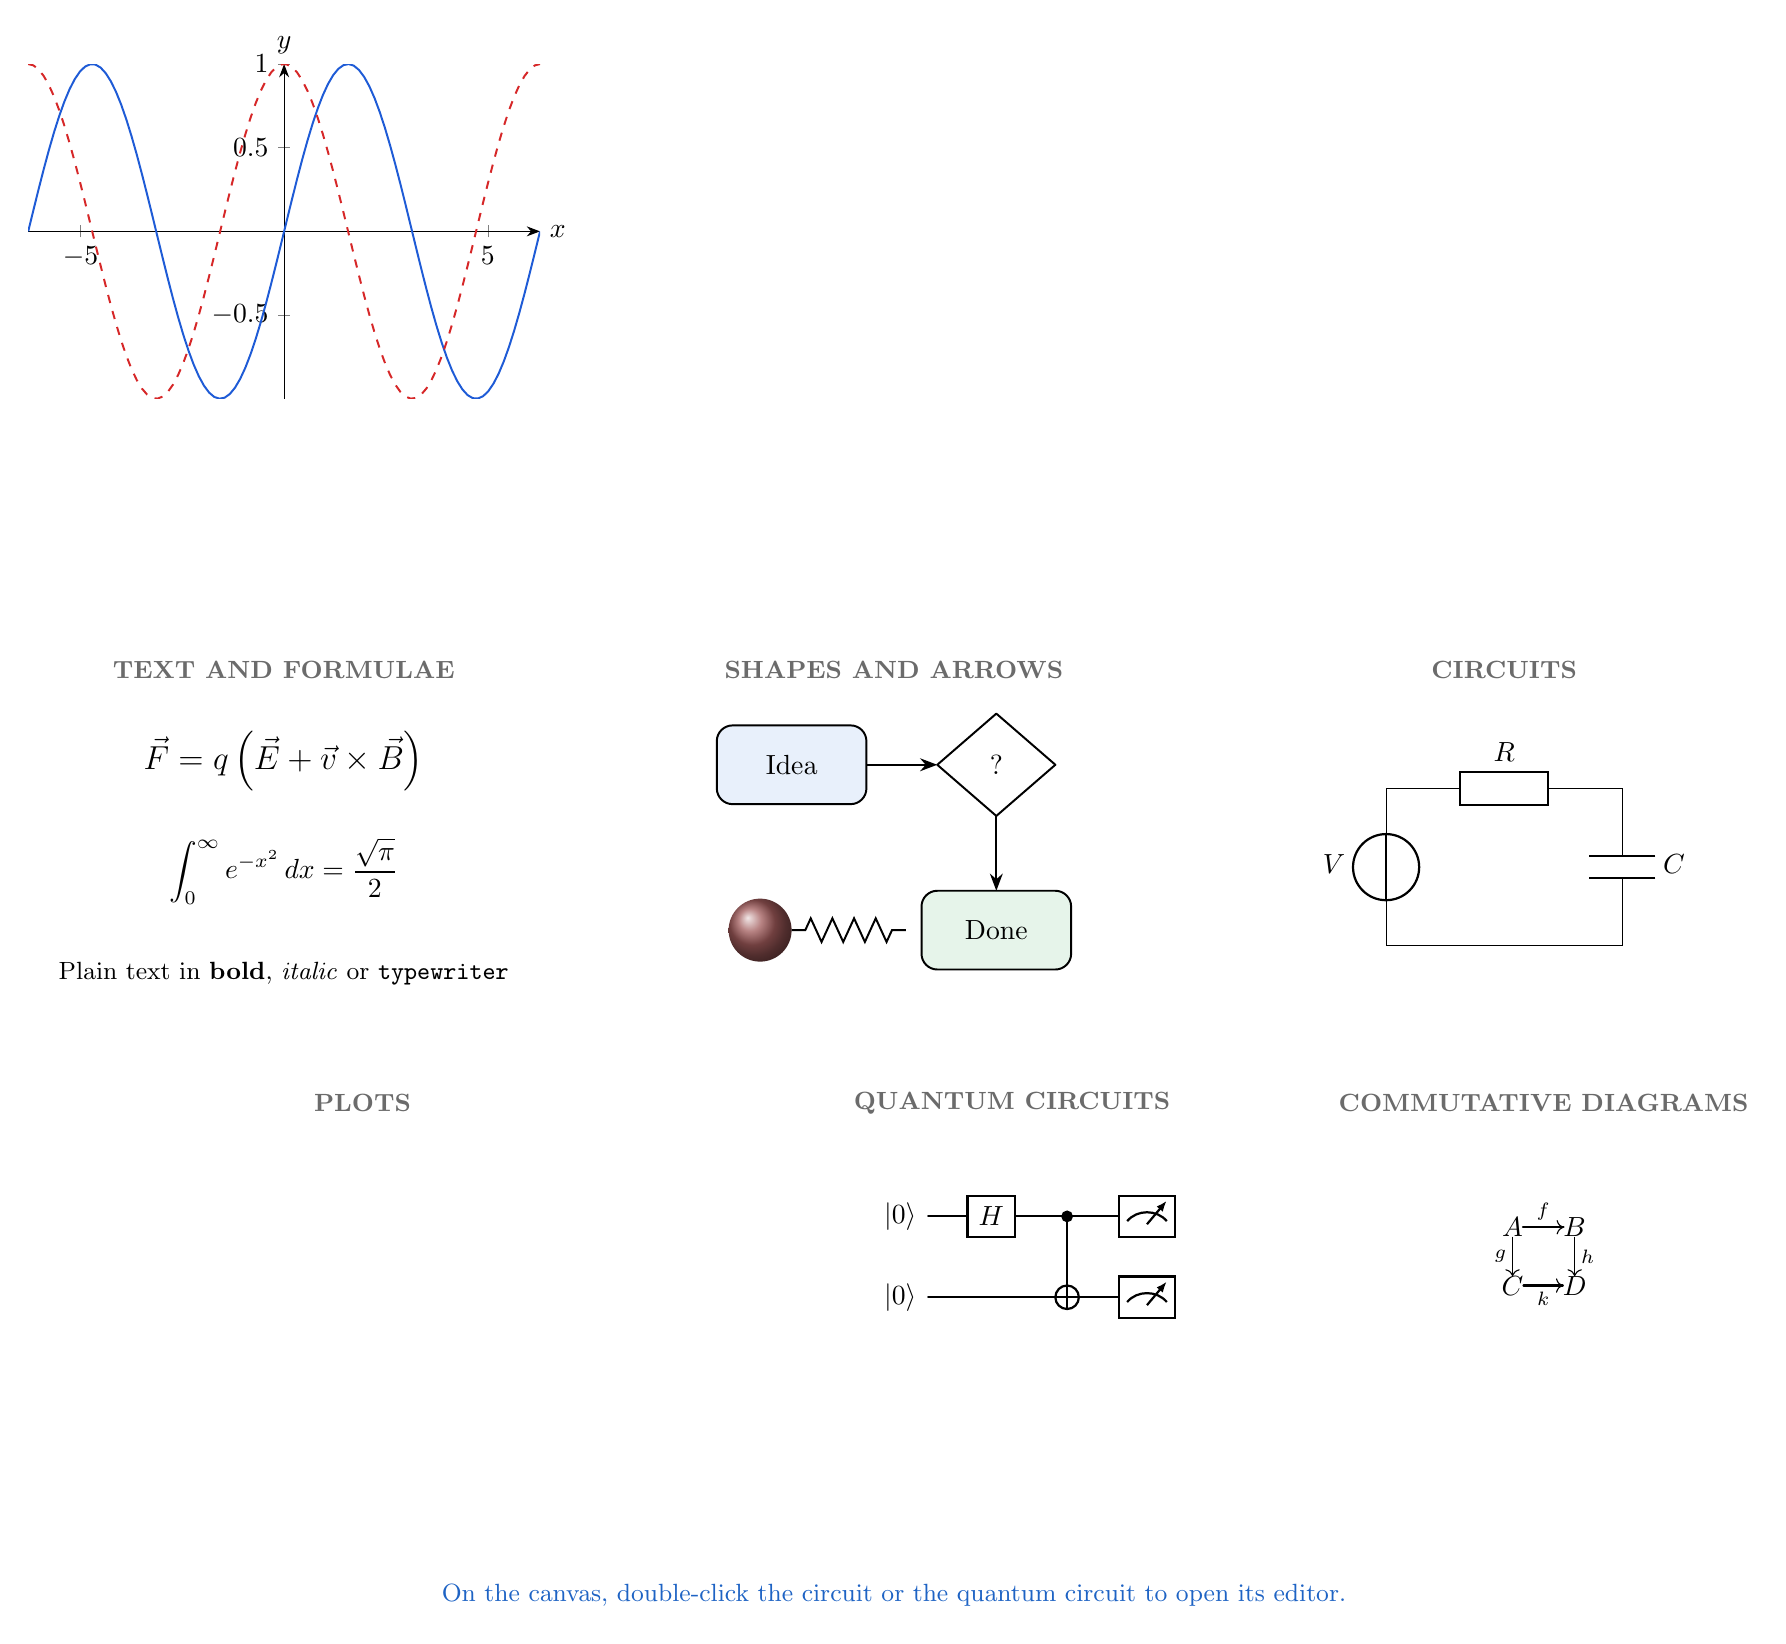
\begin{tikzpicture}[x=1cm, y=1cm]
  % diagramtex-data: W3sidHlwZSI6InRleHQiLCJ4IjoxMzAsInkiOjE1MCwidGV4dCI6IlRFWFQgQU5EIEZPUk1VTEFFIiwidHciOjAsInNpemUiOiJzbWFsbCIsImZvbnQiOiJkZWZhdWx0IiwiYm9sZCI6dHJ1ZSwiaXRhbGljIjpmYWxzZSwiY29sb3IiOiIjNmI2YjZiIiwib3BhY2l0eSI6MX0seyJ0eXBlIjoidGV4dCIsIngiOjEzMCwieSI6MTk2LCJ0ZXh0IjoiJFxcdmVjIEYgPSBxXFxsZWZ0KFxcdmVjIEUgKyBcXHZlYyB2IFxcdGltZXMgXFx2ZWMgQlxccmlnaHQpJCIsInR3IjowLCJzaXplIjoibGFyZ2UiLCJmb250IjoiZGVmYXVsdCIsImJvbGQiOmZhbHNlLCJpdGFsaWMiOmZhbHNlLCJjb2xvciI6IiMwMDAwMDAiLCJvcGFjaXR5IjoxfSx7InR5cGUiOiJ0ZXh0IiwieCI6MTMwLCJ5IjoyNTIsInRleHQiOiIkXFxkaXNwbGF5c3R5bGVcXGludF8wXlxcaW5mdHkgZV57LXheMn1cXCxkeCA9IFxcZnJhY3tcXHNxcnR7XFxwaX19ezJ9JCIsInR3IjowLCJzaXplIjoibm9ybWFsc2l6ZSIsImZvbnQiOiJkZWZhdWx0IiwiYm9sZCI6ZmFsc2UsIml0YWxpYyI6ZmFsc2UsImNvbG9yIjoiIzAwMDAwMCIsIm9wYWNpdHkiOjF9LHsidHlwZSI6InRleHQiLCJ4IjoxMzAsInkiOjMwNCwidGV4dCI6IlBsYWluIHRleHQgaW4gXFx0ZXh0YmZ7Ym9sZH0sIFxcdGV4dGl0e2l0YWxpY30gb3IgXFx0ZXh0dHR7dHlwZXdyaXRlcn0iLCJ0dyI6MCwic2l6ZSI6InNtYWxsIiwiZm9udCI6ImRlZmF1bHQiLCJib2xkIjpmYWxzZSwiaXRhbGljIjpmYWxzZSwiY29sb3IiOiIjMDAwMDAwIiwib3BhY2l0eSI6MX0seyJ0eXBlIjoidGV4dCIsIngiOjQ0MCwieSI6MTUwLCJ0ZXh0IjoiU0hBUEVTIEFORCBBUlJPV1MiLCJ0dyI6MCwic2l6ZSI6InNtYWxsIiwiZm9udCI6ImRlZmF1bHQiLCJib2xkIjp0cnVlLCJpdGFsaWMiOmZhbHNlLCJjb2xvciI6IiM2YjZiNmIiLCJvcGFjaXR5IjoxfSx7InR5cGUiOiJzeW0iLCJraW5kIjoicnJlY3QiLCJ4IjozNTAsInkiOjE3OCwidyI6NzYsImgiOjQwLCJyb3QiOjAsImZ4IjpmYWxzZSwiZnkiOmZhbHNlLCJzdHJva2UiOiIjMDAwMDAwIiwid2lkdGgiOjEsImRhc2giOiJzb2xpZCIsIm9wYWNpdHkiOjEsImZpbGwiOiIjZThmMGZiIiwiYW5nbGUiOjAsInNrZXciOjAsInRleHQiOiJJZGVhIiwic2l6ZSI6Im5vcm1hbHNpemUiLCJmb250IjoiZGVmYXVsdCIsImJvbGQiOmZhbHNlLCJpdGFsaWMiOmZhbHNlLCJjb2xvciI6IiMwMDAwMDAifSx7InR5cGUiOiJsaW5lIiwieDEiOjQyNiwieTEiOjE5OCwieDIiOjQ2MiwieTIiOjE5OCwic3Ryb2tlIjoiIzAwMDAwMCIsIndpZHRoIjoxLCJkYXNoIjoic29saWQiLCJvcGFjaXR5IjoxLCJzdGFydFRpcCI6Im5vbmUiLCJlbmRUaXAiOiJzdGVhbHRoIiwibWlkVGlwIjoibm9uZSIsInNoYWZ0Ijoic2luZ2xlIiwiY3Jvc3MiOiJub25lIiwibGFiZWwiOiIiLCJsYWJlbFBvcyI6MC41LCJsYWJlbFNpZGUiOiJsZWZ0Iiwic2l6ZSI6Im5vcm1hbHNpemUiLCJmb250IjoiZGVmYXVsdCIsImJvbGQiOmZhbHNlLCJpdGFsaWMiOmZhbHNlLCJjb2xvciI6IiMwMDAwMDAifSx7InR5cGUiOiJzeW0iLCJraW5kIjoiZGlhbW9uZCIsIngiOjQ2MiwieSI6MTcyLCJ3Ijo2MCwiaCI6NTIsInJvdCI6MCwiZngiOmZhbHNlLCJmeSI6ZmFsc2UsInN0cm9rZSI6IiMwMDAwMDAiLCJ3aWR0aCI6MSwiZGFzaCI6InNvbGlkIiwib3BhY2l0eSI6MSwiZmlsbCI6bnVsbCwiYW5nbGUiOjAsInNrZXciOjAsInRleHQiOiIkPyQiLCJzaXplIjoibm9ybWFsc2l6ZSIsImZvbnQiOiJkZWZhdWx0IiwiYm9sZCI6ZmFsc2UsIml0YWxpYyI6ZmFsc2UsImNvbG9yIjoiIzAwMDAwMCJ9LHsidHlwZSI6ImxpbmUiLCJ4MSI6NDkyLCJ5MSI6MjI0LCJ4MiI6NDkyLCJ5MiI6MjYyLCJzdHJva2UiOiIjMDAwMDAwIiwid2lkdGgiOjEsImRhc2giOiJzb2xpZCIsIm9wYWNpdHkiOjEsInN0YXJ0VGlwIjoibm9uZSIsImVuZFRpcCI6InN0ZWFsdGgiLCJtaWRUaXAiOiJub25lIiwic2hhZnQiOiJzaW5nbGUiLCJjcm9zcyI6Im5vbmUiLCJsYWJlbCI6IiIsImxhYmVsUG9zIjowLjUsImxhYmVsU2lkZSI6ImxlZnQiLCJzaXplIjoibm9ybWFsc2l6ZSIsImZvbnQiOiJkZWZhdWx0IiwiYm9sZCI6ZmFsc2UsIml0YWxpYyI6ZmFsc2UsImNvbG9yIjoiIzAwMDAwMCJ9LHsidHlwZSI6InN5bSIsImtpbmQiOiJycmVjdCIsIngiOjQ1NCwieSI6MjYyLCJ3Ijo3NiwiaCI6NDAsInJvdCI6MCwiZngiOmZhbHNlLCJmeSI6ZmFsc2UsInN0cm9rZSI6IiMwMDAwMDAiLCJ3aWR0aCI6MSwiZGFzaCI6InNvbGlkIiwib3BhY2l0eSI6MSwiZmlsbCI6IiNlNmY0ZWEiLCJhbmdsZSI6MCwic2tldyI6MCwidGV4dCI6IkRvbmUiLCJzaXplIjoibm9ybWFsc2l6ZSIsImZvbnQiOiJkZWZhdWx0IiwiYm9sZCI6ZmFsc2UsIml0YWxpYyI6ZmFsc2UsImNvbG9yIjoiIzAwMDAwMCJ9LHsidHlwZSI6ImJhbGwiLCJjeCI6MzcyLCJjeSI6MjgyLCJyIjoxNiwiYmFsbENvbG9yIjoiI2EwNWE1YSIsIm9wYWNpdHkiOjF9LHsidHlwZSI6InNwcmluZyIsIngxIjozODgsInkxIjoyODIsIngyIjo0NDYsInkyIjoyODIsInBpdGNoIjoxMiwiYW1wbGl0dWRlIjo2LCJzdHJva2UiOiIjMDAwMDAwIiwid2lkdGgiOjEsImRhc2giOiJzb2xpZCIsIm9wYWNpdHkiOjF9LHsidHlwZSI6InRleHQiLCJ4Ijo3NTAsInkiOjE1MCwidGV4dCI6IkNJUkNVSVRTIiwidHciOjAsInNpemUiOiJzbWFsbCIsImZvbnQiOiJkZWZhdWx0IiwiYm9sZCI6dHJ1ZSwiaXRhbGljIjpmYWxzZSwiY29sb3IiOiIjNmI2YjZiIiwib3BhY2l0eSI6MX0seyJ0eXBlIjoiY3oiLCJ4Ijo2OTAsInkiOjI5MCwiaXRlbXMiOlt7ImlkIjoidThpZmRwdHAiLCJwYXJ0Ijoic3JjOnZzb3VyY2UtZXUiLCJhIjpbMCwwXSwiYiI6WzAsMl0sImwiOiIkViQiLCJhbm4iOiIiLCJ2IjoiIiwiaSI6IiIsInBvbGVzIjoiIiwibmFtZSI6IiIsIm9wdHMiOiIifSx7ImlkIjoiM2VhcG14OHMiLCJwYXJ0IjoicmVzOmllYyIsImEiOlswLDJdLCJiIjpbMywyXSwibCI6IiRSJCIsImFubiI6IiIsInYiOiIiLCJpIjoiIiwicG9sZXMiOiIiLCJuYW1lIjoiIiwib3B0cyI6IiJ9LHsiaWQiOiJ3M2hyMDluOSIsInBhcnQiOiJjYXA6aWVjIiwiYSI6WzMsMl0sImIiOlszLDBdLCJsIjoiJEMkIiwiYW5uIjoiIiwidiI6IiIsImkiOiIiLCJwb2xlcyI6IiIsIm5hbWUiOiIiLCJvcHRzIjoiIn0seyJpZCI6IjVzeW5nOTRsIiwicGFydCI6InNob3J0IiwiYSI6WzMsMF0sImIiOlswLDBdLCJsIjoiIiwiYW5uIjoiIiwidiI6IiIsImkiOiIiLCJwb2xlcyI6IiIsIm5hbWUiOiIiLCJvcHRzIjoiIn1dLCJyYXciOiIiLCJzaXplIjoibGFyZ2UiLCJmb250IjoiZGVmYXVsdCIsImNvbG9yIjoiIzAwMDAwMCJ9LHsidHlwZSI6InRleHQiLCJ4IjoxNzAsInkiOjM3MCwidGV4dCI6IlBMT1RTIiwidHciOjAsInNpemUiOiJzbWFsbCIsImZvbnQiOiJkZWZhdWx0IiwiYm9sZCI6dHJ1ZSwiaXRhbGljIjpmYWxzZSwiY29sb3IiOiIjNmI2YjZiIiwib3BhY2l0eSI6MX0seyJ0eXBlIjoicGxvdCIsIngiOjQwLCJ5IjozOTYsInciOjI2MCwiaCI6MTcwLCJkaW0iOjIsInRpdGxlIjoiIiwieGxhYmVsIjoiJHgkIiwieWxhYmVsIjoiJHkkIiwiemxhYmVsIjoiIiwiYXhpc0xpbmVzIjoibWlkZGxlIiwiZ3JpZCI6ZmFsc2UsInhtaW4iOiIiLCJ4bWF4IjoiIiwieW1pbiI6IiIsInltYXgiOiIiLCJ6bWluIjoiIiwiem1heCI6IiIsInZpZXciOlsyNSwzMF0sImNvbG9ybWFwIjoiaG90IiwiY29sb3JiYXIiOmZhbHNlLCJsZWdlbmRQb3MiOiJub3J0aCBlYXN0Iiwic2VyaWVzIjpbeyJraW5kIjoibGluZSIsInNvdXJjZSI6ImV4cHIiLCJleHByIjoic2luKHgpIiwiZGF0YSI6IiIsImRvbWFpbiI6WyItMipwaSIsIjIqcGkiXSwieWRvbWFpbiI6WyItNSIsIjUiXSwic2FtcGxlcyI6MTAwLCJjb2xvciI6IiMxZTViZDYiLCJ3aWR0aCI6MSwiZGFzaCI6InNvbGlkIiwibWFyayI6Im5vbmUiLCJsZWdlbmQiOiIiLCJsZXZlbHMiOjgsImJhcldpZHRoIjoxMiwib3BhY2l0eSI6MX0seyJraW5kIjoibGluZSIsInNvdXJjZSI6ImV4cHIiLCJleHByIjoiY29zKHgpIiwiZGF0YSI6IiIsImRvbWFpbiI6WyItMipwaSIsIjIqcGkiXSwieWRvbWFpbiI6WyItNSIsIjUiXSwic2FtcGxlcyI6MTAwLCJjb2xvciI6IiNkNjI3MjgiLCJ3aWR0aCI6MSwiZGFzaCI6ImRhc2hlZCIsIm1hcmsiOiJub25lIiwibGVnZW5kIjoiIiwibGV2ZWxzIjo4LCJiYXJXaWR0aCI6MTIsIm9wYWNpdHkiOjF9XSwiX3B3IjoyODAsIl9waCI6MjAwfSx7InR5cGUiOiJ0ZXh0IiwieCI6NTAwLCJ5IjozNzAsInRleHQiOiJRVUFOVFVNIENJUkNVSVRTIiwidHciOjAsInNpemUiOiJzbWFsbCIsImZvbnQiOiJkZWZhdWx0IiwiYm9sZCI6dHJ1ZSwiaXRhbGljIjpmYWxzZSwiY29sb3IiOiIjNmI2YjZiIiwib3BhY2l0eSI6MX0seyJ0eXBlIjoicWMiLCJ4Ijo0MjgsInkiOjQxMCwic3JjIjoiXFxiZWdpbntxdWFudGlren1cblxcbHN0aWNre1xca2V0ezB9fSAmIFxcZ2F0ZXtIfSAmIFxcY3RybHsxfSAmIFxcbWV0ZXJ7fSBcXFxcXG5cXGxzdGlja3tcXGtldHswfX0gJiAmIFxcdGFyZ3t9ICYgXFxtZXRlcnt9XG5cXGVuZHtxdWFudGlren0iLCJzaXplIjoibGFyZ2UiLCJmb250IjoiZGVmYXVsdCIsImNvbG9yIjoiIzAwMDAwMCJ9LHsidHlwZSI6InRleHQiLCJ4Ijo3NzAsInkiOjM3MCwidGV4dCI6IkNPTU1VVEFUSVZFIERJQUdSQU1TIiwidHciOjAsInNpemUiOiJzbWFsbCIsImZvbnQiOiJkZWZhdWx0IiwiYm9sZCI6dHJ1ZSwiaXRhbGljIjpmYWxzZSwiY29sb3IiOiIjNmI2YjZiIiwib3BhY2l0eSI6MX0seyJ0eXBlIjoiY2QiLCJ4Ijo3MzAsInkiOjQxMCwic3JjIjoiXFxiZWdpbnt0aWt6Y2R9XG4gIEEgXFxhcnJvd1tyLCBcImZcIl0gXFxhcnJvd1tkLCBcImdcIiddICYgQiBcXGFycm93W2QsIFwiaFwiXSBcXFxcXG4gIEMgXFxhcnJvd1tyLCBcImtcIiddICAgICAgICAgICAgICAgICAgJiBEXG5cXGVuZHt0aWt6Y2R9IiwiY29sb3IiOiIjMDAwMDAwIn0seyJ0eXBlIjoidGV4dCIsIngiOjQ0MCwieSI6NjIwLCJ0ZXh0IjoiT24gdGhlIGNhbnZhcywgZG91YmxlLWNsaWNrIHRoZSBjaXJjdWl0IG9yIHRoZSBxdWFudHVtIGNpcmN1aXQgdG8gb3BlbiBpdHMgZWRpdG9yLiIsInR3IjowLCJzaXplIjoic21hbGwiLCJmb250IjoiZGVmYXVsdCIsImJvbGQiOmZhbHNlLCJpdGFsaWMiOmZhbHNlLCJjb2xvciI6IiMxZTYzYzQiLCJvcGFjaXR5IjoxfV0=
  \node[font=\small\bfseries, text=tdc1] at (3.25,-3.75) {TEXT AND FORMULAE};
  \node[font=\large] at (3.25,-4.9) {$\vec F = q\left(\vec E + \vec v \times \vec B\right)$};
  \node at (3.25,-6.3) {$\displaystyle\int_0^\infty e^{-x^2}\,dx = \frac{\sqrt{\pi}}{2}$};
  \node[font=\small] at (3.25,-7.6) {Plain text in \textbf{bold}, \textit{italic} or \texttt{typewriter}};
  \node[font=\small\bfseries, text=tdc1] at (11,-3.75) {SHAPES AND ARROWS};
  \draw[line width=0.71pt, fill=tdc2, line join=round] (8.95,-4.45) -- (10.45,-4.45) -- (10.45,-4.45) .. controls (10.56,-4.45) and (10.65,-4.54) .. (10.65,-4.65) -- (10.65,-5.25) -- (10.65,-5.25) .. controls (10.65,-5.36) and (10.56,-5.45) .. (10.45,-5.45) -- (8.95,-5.45) -- (8.95,-5.45) .. controls (8.84,-5.45) and (8.75,-5.36) .. (8.75,-5.25) -- (8.75,-4.65) -- (8.75,-4.65) .. controls (8.75,-4.54) and (8.84,-4.45) .. (8.95,-4.45) -- cycle;
  \node[align=center] at (9.7,-4.95) {Idea};
  \draw[line width=0.71pt, -{Stealth}] (10.65,-4.95) -- (11.55,-4.95);
  \draw[line width=0.71pt, line join=round] (12.3,-4.3) -- (13.05,-4.95) -- (12.3,-5.6) -- (11.55,-4.95) -- cycle;
  \node[align=center] at (12.3,-4.95) {$?$};
  \draw[line width=0.71pt, -{Stealth}] (12.3,-5.6) -- (12.3,-6.55);
  \draw[line width=0.71pt, fill=tdc3, line join=round] (11.55,-6.55) -- (13.05,-6.55) -- (13.05,-6.55) .. controls (13.16,-6.55) and (13.25,-6.64) .. (13.25,-6.75) -- (13.25,-7.35) -- (13.25,-7.35) .. controls (13.25,-7.46) and (13.16,-7.55) .. (13.05,-7.55) -- (11.55,-7.55) -- (11.55,-7.55) .. controls (11.44,-7.55) and (11.35,-7.46) .. (11.35,-7.35) -- (11.35,-6.75) -- (11.35,-6.75) .. controls (11.35,-6.64) and (11.44,-6.55) .. (11.55,-6.55) -- cycle;
  \node[align=center] at (12.3,-7.05) {Done};
  \shade[ball color=tdc4] (9.3,-7.05) circle (0.4);
  \draw[line width=0.71pt, decorate, decoration={zigzag, segment length=0.2752cm, amplitude=0.15cm, pre length=0.174cm, post length=0.174cm}] (9.7,-7.05) -- (11.15,-7.05);
  \node[font=\small\bfseries, text=tdc1] at (18.75,-3.75) {CIRCUITS};
  \begin{scope}[shift={(17.25,-7.25)}]
    \draw (0,0) to[european voltage source, l=$V$] (0,2);
    \draw (0,2) to[european resistor, l=$R$] (3,2);
    \draw (3,2) to[capacitor, l=$C$] (3,0);
    \draw (3,0) -- (0,0);
  \end{scope}
  \node[font=\small\bfseries, text=tdc1] at (4.25,-9.25) {PLOTS};
  \begin{axis}[
    at={(1,-14.15)},
    anchor=south west,
    scale only axis,
    width=6.5cm,
    height=4.25cm,
    xmin=-6.2832,
    xmax=6.2832,
    ymin=-0.9999,
    ymax=1,
    xtick={-5,0,5},
    ytick={-0.5,0,0.5,1},
    axis lines=middle,
    axis line style={-{Stealth}},
    every axis x label/.style={at={(current axis.right of origin)}, anchor=west},
    every axis y label/.style={at={(current axis.above origin)}, anchor=south},
    xlabel={$x$},
    ylabel={$y$}
  ]
    \addplot[color=tdc5, line width=0.71pt, no marks, domain=-6.2832:6.2832, samples=100, forget plot] {sin(deg(x))};
    \addplot[color=tdc6, line width=0.71pt, dashed, no marks, domain=-6.2832:6.2832, samples=100, forget plot] {cos(deg(x))};
  \end{axis}
  \node[font=\small\bfseries, text=tdc1] at (12.5,-9.25) {QUANTUM CIRCUITS};
  \node at (12.72,-11.13) {\pgfinterruptpicture%
  \begin{quantikz}
  \lstick{\ket{0}} & \gate{H} & \ctrl{1} & \meter{} \\
  \lstick{\ket{0}} & & \targ{} & \meter{}
  \end{quantikz}%
  \endpgfinterruptpicture};
  \node[font=\small\bfseries, text=tdc1] at (19.25,-9.25) {COMMUTATIVE DIAGRAMS};
  \node at (19.26,-11.17) {\pgfinterruptpicture%
  \begin{tikzcd}
    A \arrow[r, "f"] \arrow[d, "g"'] & B \arrow[d, "h"] \\
    C \arrow[r, "k"']                  & D
  \end{tikzcd}%
  \endpgfinterruptpicture};
  \node[font=\small, text=tdc7] at (11,-15.5) {On the canvas, double-click the circuit or the quantum circuit to open its editor.};
\end{tikzpicture}
}
\end{center}

\section*{How to use}
\begin{itemize}
  \item Draw with the tools on the left; \textbf{Plots} and \textbf{Blocks} hold graphs, circuits and more.
  \item Double-click to edit, right-click for more. Maths goes between \$ signs.
  \item In Classic, switch between \textbf{Document} and \textbf{Diagram} at the top, or double-click a diagram.
  \item \textbf{Code} gives TikZ, \textbf{LaTeX} the whole document, \textbf{Export} a picture or PDF.
\end{itemize}

\end{document}
